\section{Entscheidungsbäume, Boosting und Bagging}
\textit{Annalena Gutheil, Matthias Volland}

\subsection{Einführung}
Entscheidungsbäume besitzen eine baumartige, hierarchische Struktur, bestehend aus Knoten, Kanten und Blättern. 
Bei der Klassifikation entsprechen die Knoten den Datenmerkmalen und die Blätter den Klassen. 
Entscheidungsbäume funktionieren nach dem \glqq teile und herrsche\grqq -Prinzip. 
Beginnend beim Wurzelknoten wird bei jedem Knoten mithilfe einer Testfunktion berechnet, 
welche Abzweigung genommen werden muss. 
Ist man am Blattknoten angekommen, ist dies die zur Eingabe gehörende Klasse~\cite{alpaydin:maschinelles_lernen, borgelt:data_mining}.

\subsubsection*{Random Forests}

Die Besonderheit von Ensemble Learning ist, dass mit Hilfe von vielen schwachen Klassifikatoren 
gute Klassifikationsergebnisse erzielt werden können. 
Die Entscheidungen, die die verschiedenen Klassifikatoren treffen, sind dabei verschieden, 
was jedoch auch die Stärke dieser Methode ist, denn sie ergänzen sich gegenseitig

\subsection{Datenaufbereitung}

Die zu klassifizierenden Gesten unterscheiden sich dahingehend, dass sie die Bandbreite 
des Frequenzspektrums um den Referenzton in unterschiedlicher Weise verschieben bzw. vergrößern. 
Um eine Geste zu erkennen, werden daher die Amplituden der aufgezeichneten Frequenzen 
um die Amplitude der Frequenz des Referenztons im Spektrum in beiden Richtungen analysiert. 
Relevant für die Erkennung der Gesten sind dabei im Allgemeinen nur diejenigen Frequenzanteile 
um den Referenzton, deren Amplitude den Grenzwert von 10\% der Amplitude des Referenztones nicht unterschreitet. 
In Ausnahmefällen können die Frequenzanteile einer Geste im Spektrum durch ein lokales Minimum vom Referenzton 
separiert sein. Daher wird zusätzlich nach einem weiteren Ausschlag im Spektrum gesucht, 
dessen Maximum mindestens 30\% der Amplitude des Referenztons entsprechen muss.


Eine Geste setzt sich zunächst aus 32 Einzelaufnahmen (Samples) zusammen, welche jeweils 
64 Amplitudenwerte beinhalten. Somit besteht eine Geste zunächst aus insgesamt 2048 Werten.
Da wie einführend beschrieben die Frequenzanteile einer Geste durch ein lokales Minimum vom Referenzton 
getrennt sein können, werden die einzelnen Samples zunächst mit einem Gauß-Filter geglättet. 
Die folgende Abbildung zeigt die Amplituden des Frequenzspektrums von einem Sample 
vor dem Glätten mit einem Gauß-Filter (rot) und danach (blau).

\begin{center}
  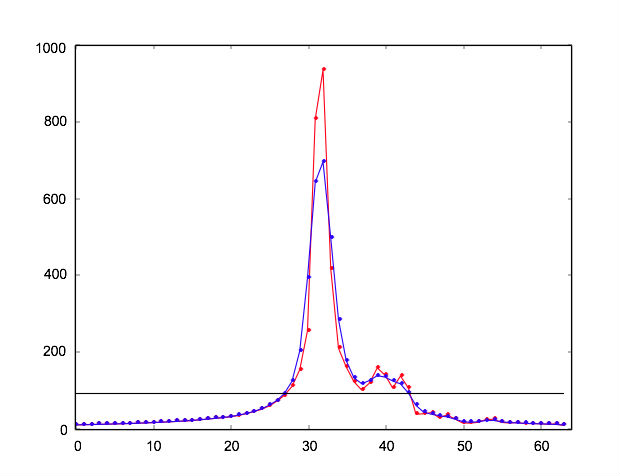
\includegraphics[height=60mm]{trees/gesture4-gauss1.jpg}
\end{center}

Für die effiziente und robuste Klassifizierung der Gesten bietet es sich weiterhin an, 
die Komplexität der generierten Eingabedaten zu reduzieren. Dazu wird in jedem Sample einer Geste 
auf der linken und rechten Seite des Referenztons die Anzahl der Amplituden des geglätteten Signals ermittelt, 
deren Wert größer als 10\% ist. Der daraus resultierende Graph zeigt dann für eine Geste die zeitliche 
Änderung der Amplitudenanteile um den Referenzton auf der linken und rechten Seite an. Dieser Graph ist in der folgenden 
Abbildung dargestellt, wobei die Anzahl der zum Referenzton gehörenden Amplituden aller Frequenzen unterhalb des
Referenztons in rot dargestellt sind, die Frequenzanteile oberhalb des Referenztons in blau:

\begin{center}
  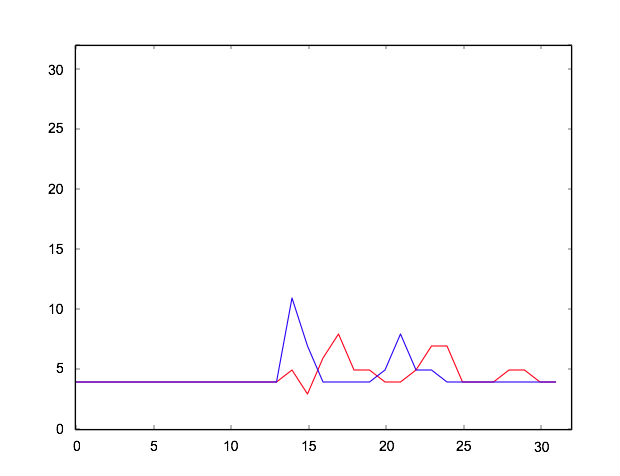
\includegraphics[height=60mm]{trees/gesture4-peaksize.jpg}
\end{center}

Bei der in der Grafik dargestellten Geste handelt es sich um einen \glqq Double-Tap\grqq , also eine Geste, bei der die Hand zwei mal 
hintereinander schnell auf den Monitor bzw. das Mikrofon zubewegt wird. Diese Geste äußert sich in jeweils zwei aufeinander folgenden 
Verschiebungen der Frequenzen nach rechts (auf den Monitor zu bewegen) und links (vom Monitor weg bewegen). 
Diese Charakteristik lässt sich in der Grafik erkennen, da die Anzahl der zum Referenzton gehörenden Frequenzanteile zunächst nach rechts (erster Peak blau) und dann nach links (zweiter Peak rot) ansteigt. Aufgrund des \glqq Double-Tap\grqq  erfolgt diese 
Verschiebung zwei mal hintereinander, so dass insgesamt vier Ausschläge (zwei nach rechts und zwei nach links) zu erkennen sind. 
Somit kann in einem Schritt die Anzahl der Daten pro zu klassifizierender Geste von 32*64=2048 Amplitudenwerten 
auf 2*32=64 reduziert werden, wobei diese Werte keinen Rückschluss auf die genauen Frequenzanteile zulassen sondern 
ein Maß dafür sind, wie sich die Frequenzanteile ober- und unterhalb des Referenztons verändern.

Die daraus entstehenden Daten können in einem weiteren Schritt geglättet werden, da nur Amplitudenschwankungen ab einer gewissen 
Größe auf eine ausgeführte Bewegung schließen lassen. Dazu werden alle Schwankungen auf der rechten oder linken Seite entfernt, 
die unterhalb eines definierten Grenzwertes liegen. 
Die folgende Abbildung zeigt ein gefilterten Graph, in dem alle Ausschläge entfernt werden, die kleiner als 2 sind:

\begin{center}
  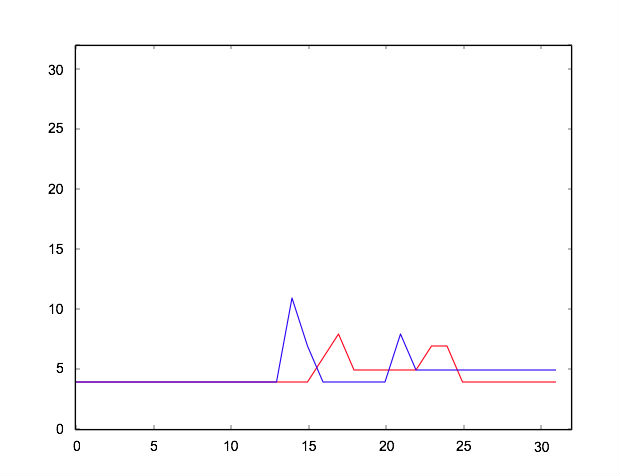
\includegraphics[height=60mm]{trees/gesture4-peaksize-smoothed.jpg}
\end{center}

Mit einen dritten Schritt werden die Amplitudenwechsel dahingehend weiter geglättet, indem zunächst die Anzahl der am häufigsten 
auftretenden Frequenzanteile auf der linken und rechten Seite vom Referenzton ermittelt werden. Anschließend werden alle Werte,
die in einem vorher definierten Bereich ober- oder unterhalb dieses Wertes liegen auf den am häufigsten vorkommenden Wert gesetzt.
Dieser Schritt ist in der folgenden Abbildung zu sehen, wobei alle Werte die +1 oder -1 um den häufigsten Wert verteilt sind 
auf den häufigsten Wert gesetzt wurden:

\begin{center}
  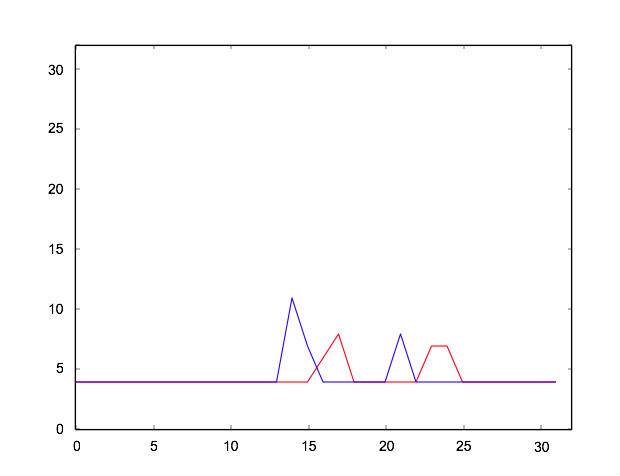
\includegraphics[height=60mm]{trees/gesture4-peaksize-smoothed2.jpg}
\end{center}


Stark vereinfacht unterscheiden sich die Gesten dahingehend, ob und auf welcher Seite 
eine Veränderung der Anzahl aller zum Referenzton gehörenden Frequenzanteile stattfindet. 
Weiterhin muss unterschieden werden, in welche Richtung sich diese Verschiebung ausbreitet. 
Sie kann beispielsweise von der rechten zur linken oder von der linken zur rechten Seite 
um den Referenzton wandern, sowie vom Referenzton beginnend in eine Richtung ausschlagen. 
Diese Unterscheidungsmerkmale können sehr gut durch einen Entscheidungsbaum abgebildet werden. 
Dazu kann die Verschiebungsrichtung als Maß dienen, um die Eingabemenge zu unterteilen und 
somit eine Klassifizierung zu erreichen.


\subsection{Klassifikator}

\subsection{Implementierung}
Die Bibliothek \textit{sklearn}~\cite{sklearn} stellt mit dem Modul \textit{sklearn.ensemble}~\cite{sklearn.ensemble} einige hilfreiche Klassen und Methoden zur Klassifikation bereit.

\subsection{Training}

\subsection{Evaluation}

\subsection{Fazit}


